\documentclass{article}
\usepackage[all]{xy}
\usepackage{graphicx}
\usepackage{amsmath}
\usepackage{amssymb}
\usepackage{cite}
\usepackage{tikz}
\usepackage{tikz-3dplot}

\addtolength{\oddsidemargin}{-.5in}
\addtolength{\evensidemargin}{-.5in}
\addtolength{\textwidth}{1in}
\title{Caliber v1.0 Manual}
\author{Albert Liu}



\begin{document}
\maketitle
\tableofcontents
\newpage
\part{Tutorial}
\section{Introduction}
\subsection{Purpose}

One way to think of Caliber is as as camera calibration system. Consider the 
calibration of a single conventional camera using known feature points.

The basic single-camera problem can be described as follows: Suppose we have a set of images from 
a single camera of a set of worldspace points (a \textit{pointset}). The  
relationships of the points in the pointset to each other are known--for 
example, the grid intersections of a checkerboard of known square size. 
Using this information, and the corresponding image features in the photographs, 
we can answer the following 
questions:
\begin{itemize}
	\item What are the \textit{intrinsics} of the camera? These include the following:
		\begin{itemize}
			\item The \textit{focal length} of the camera in pixels. 
				For digital cameras, this is determined
				by the resolution and field of view (modulo any distortion).
			\item The \textit{principal point} of the camera. This is the point in the image
				that matches where the camera is ``pointing'', which may not be exactly the 
				same as the center of the image (though it is usually close).
			\item The \textit{distortion} of the camera. In particular, \textit{radial distortion}
				is often of interest, and is modeled as a displacement of image points
				by an even polynomial relative to an undistorted image. The (first few)
				coefficients of this polynomial are then taken to describe the radial distortion.
		\end{itemize}
	\item What are the \textit{extrinsics} of the camera? These can be described using a linear 
			\textit{transformation} matrix.
		\begin{itemize}
			\item What is the position of the camera center relative to each pointset?
			\item What is the orientation of the camera relative to each pointset?
		\end{itemize}
\end{itemize}
We can characterize the quality of a solution to these questions by comparing the image points 
the solution predicts to the actual observed image points. This is called \textit{reprojection error};
taking the reprojection error over all image points allows us to define an objective function, and
thus a definition of an optimal solution in a least-squares sense.

The problem of finding this optimal solution is well-studied, resulting in such systems as 
Bouguet's popular calibration toolbox \\
(\texttt{http://www.vision.caltech.edu/bouguetj/calib\_doc/}).
However, more complex scenarios can easily be envisioned. For example:

\begin{itemize}
	\item What if there are multiple cameras, and something is known about their relative geometry?
	\item What if more than one pointset appears in a single image?
	\item What if the camera(s) and/or pointset(s) are mounted on robot arms, where the mounting 
		transformation is unknown, but the arm transformations are known?
	\item What if there are multiple devices with both cameras and pointsets 
		(e.g. laptop or tablet computers that have integral cameras and are capable of displaying
		an image of a checkerboard on their screens)?
\end{itemize}

We could use single-camera calibration on each camera independently to calibrate these scenarios. 
However, this approach has a couple major shortcomings:
\begin{itemize}
	\item These known constraints on the extrinsics cannot be expressed directly, 
		and thus the solution may violate these constraints. 
	\item If the constraints are applied after the fact, the solution may 
		no longer be optimal.
	\item A satisfactory process of applying the constraints after the fact may be non-obvious 
		and/or tedious to determine, especially for complex or novel scenarios.
	\item Transformations that do not correspond directly to observations (e.g. between
		two pointsets, two cameras, a camera and a robot joint, etc.) cannot be determined directly.
		Again, it may be non-obvious and/or tedious to determine these transformations,
		especially in an optimal sense.
\end{itemize}

This is the purpose of Caliber. It allows the user to input a set of single-camera calibrations 
and a description of constraints, and produces an optimal solution that respects those constraints,
as well as values for all transformations.

\subsection{Requirements}
In addition to the Caliber code itself, you will need the following to perform a calibration:
\begin{itemize}
	\item MATLAB 7.7 (R2008b) or later. (This implementation uses the \texttt{containers.Map} class.)
		The Parallel Computing Toolbox will help speed up computations.
	\item Estimated intrinsic parameters for all cameras: 
		focal length, principal point, radial distortion coefficients.
	\item Estimated relative camera-pointset extrinsics (poses) for each image.
	\item Knowledge about the geometric structure of the system, expressed in a tree structure.
	\item If you wish to calibrate a non-conventional camera, you will need to implement its
		projection function and its Jacobian.
		as an extension of the \texttt{Observation} abstract class.
\end{itemize}
The intrinsics and extrinsics can be generated using Bouguet's calibration toolbox \\
(\texttt{http://www.vision.caltech.edu/bouguetj/calib\_doc/}). If you have a different calibration system
that can produce similar data, that can be used as well, though at current Caliber only has specific code
for Bouguet.

\section{Tree structure}

In Caliber, the constraints on the extrinsics are expressed using a tree structure. A tree
is constructed as follows:

\begin{itemize}
	\item The tree has an implicit root node, representing the ``laboratory frame'' of the system.
	\item The user adds nodes to the tree. Each node may represent a camera, pointset, or robot joint.
		For example, if a camera is mounted on a robot arm, you might attach a node representing
		the robot arm to the root, then attach a node representing the camera to that node.
	\item Each node has a number of states representing different transformations relative to its parent. 
		For example, if you moved the robot arm to three 
		different positions throughout the course of your measurements, the robot arm node would
		have three states. If the camera stayed attached the same way to the robot arm for the entire
		time, then it would have just a single state.
	\item Each state has an associated transformation, which may be known or unknown. For example,
		if your robot arm had an encoder that told you where it was relative to the root,
		each of its three states would have a known transformation. If you didn't know exactly how the
		camera was mounted on the robot arm, that camera node's (sole) 
		state would have an unknown transformation. Unknown transformations may have an initial estimate,
		or they may be completely unknown.
	\item For camera nodes, each state also has associated intrinsic information for that camera.
	\item Each state has information about which intrinsic and extrinsic parameters of that
		state are allowed to vary during the course of the optimization and which are constrained 
		to their given values.
	\item Once the tree has been defined, observations are defined by their camera and pointset nodes,
		the worldspace points in the pointset frame and their corresponding image points,
		and the state of all nodes in the tree when that photograph was taken. The optimization
		process also requires an initial estimate of the relative camera-pointset transformation,
		which can be computed by Bouguet.
\end{itemize}
\section{Examples}

In order to give a more concrete understanding, we will give some examples of calibration code.

\subsection{Stereo pair}

Our first example is a stereo pair calibration. Suppose we have ran Bouguet on the two cameras separately for each of 
$n$ images, and the results are stored in \texttt{Calib\_results1.mat} and \texttt{Calib\_results2.mat}.

First, we would read out the results from the result files:

\begin{verbatim}
indices = 1:n;
[imagePoints1, worldPoints1, Q1, data1] = ...
    caliber.io.bouguet('Calib_results1.mat', indices);
[imagePoints2, worldPoints2, Q2, data2] = ...
    caliber.io.bouguet('Calib_results2.mat', indices);
\end{verbatim}

\texttt{data1} and \texttt{data2} are structs, each containing the intrinsic information produced
by Bouguet.

Then, we can start constructing the tree. We begin by constructing a new \texttt{Tree} instance:

\begin{verbatim}
tree = caliber.tree.Tree();
\end{verbatim}

Supposing that we want to put camera1
at the origin, we would add a node for camera1:

\begin{verbatim}

tree.addNode(caliber.node.GeneralNode('camera1', [], data1, {}));
\end{verbatim}

\texttt{caliber.node.GeneralNode} is the default implementation of a Caliber node.
It allows you to specify a list of known and unknown transformations.
The first node is the root of the tree, and thus has no parent or states.

After this first node is added, our tree looks like this:

\centerline{\xymatrix{
\mathrm{camera1}
}}

Now we add camera2:

\begin{verbatim}

tree.addNode(caliber.node.GeneralNode('camera2', 'camera1', data2, {[]}));
\end{verbatim}

Here we have added a node for camera2 as a child of camera1. 
Note that the last
argument is a cell array with a single \texttt{[]} element, 
indicating that the transformation matrix is unknown, 
and that we would
like Caliber to find it. 

The tree now looks like this:

\centerline{\xymatrix{
\mathrm{camera1} \ar[d] \\
\mathrm{camera2}
}}

The last node we have to add is the pointset node:

\begin{verbatim}

tree.addNode(caliber.node.GeneralNode('pointset', 'root', struct(), cell(n)));
\end{verbatim}

Since only cameras have intrinsics, we pass an empty struct for the node's data.
Since the pointset was in a different position for each pair of photographs, its node has $n$ states.

The tree with all the nodes added looks like this:

\centerline{\xymatrix{
\mathrm{camera1} \ar[d] \ar[r] & \mathrm{pointset} \\
\mathrm{camera2}
}}

The last step before solving is to add the observations.

\begin{verbatim}
for i = 1:n
    observation = caliber.observation.IndependentObservation(...
        'camera1', 'pointset', imagePoints1{i}, worldPoints1{i},...
        Q1{i}, Map({'pointset'}, {i}));
    tree.addObservation(observation);
    observation = caliber.observation.IndependentObservation(...
        'camera2', 'pointset', imagePoints2{i}, worldPoints2{i},...
        Q2{i}, Map({'pointset'}, {i}));
    tree.addObservation(observation);
end
\end{verbatim}

We construct an observation object for each pointset state using the appropriate information,
and add those to the system. 
In this case we use \texttt{IndependentObservation}, which can represent Bouguet-style observations.
The last argument to the constructor tells Caliber that the pointset was
in state $i$ when that observation was taken. Note that only the pointset node was explicitly assigned
a state--nodes not explicitly assigned a state are assumed to be in their first state.

Pictorially, we may represent the observations as dashed arrows:

\centerline{\xymatrix{
\mathrm{camera1} \ar[d] \ar[r] & \mathrm{pointset} \\
\mathrm{camera2} \ar@{-->}[ur]
}}

Finally, we need to define the parameters of the system.

\begin{verbatim}
Kparams = logical([1 0 1; 0 1 1; 0 0 0]);
tweakSpec = {'camera1', 'K', Kparams, [];...
          'camera2', 'K', Kparams, [];...
          'camera2', {'r', 't'}, 'all', 1;...
          'pointset', {'r', 't'}, 'all', 'all'}
\end{verbatim}

The tweak argument to the solver tells Caliber which parameters of the node 
can be changed from their supplied values, which we call tweaks.
\begin{enumerate}
	\item The first element in each row indicates which node the tweak refers to.
	\item The second indicates which parameter type(s) can be tweaked.
	\item The third indicates which axes or coefficients can be tweaked.
	\item The last element, if not empty, selects which columns of the tweak data can be changed.
	For extrinsic transformations, each column corresponds to one node state.
\end{enumerate}

Here we have allowed the 
focal length and principal point axis elements of the camera matrix to
to be tweaked, as well as the extrinsic transformation matrices of the second camera and the pointset.

With this, the problem is fully defined, and we can tell Caliber to solve the problem. 

\begin{verbatim}
[initializer, optimizer] = tree.solve(tweakSpec);
\end{verbatim}

For how to retrieve and display results, see Section \ref{disp_results}.

% \input{tutorial/section_examples_xml}
\section{Retrieving and displaying results} \label{disp_results}

To get at the results, we can query the tree or the initializer and/or optimizer returned by \\
\texttt{[initializer, optimzer] = tree.solve()}.
Some examples:

\begin{verbatim}
tree.plotTree();
\end{verbatim}

This displays a pictoral representation of the tree structure--useful for double-checking
if your input is what you thought it was.
See Figure \ref{fig:tree_example} for an example of output.

\begin{figure}[t]
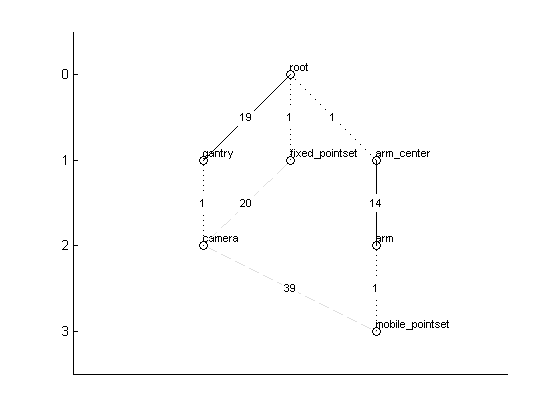
\includegraphics{figures/tree_example}
\caption{Example output for \texttt{tree.plotTree()}.}
\label{fig:tree_example}
\end{figure}

\begin{verbatim}
[x,resnorm,residual,exitflag,output,lambda,jacobian] = optimizer.lsqnonlinReturnValues{:};
\end{verbatim}

Caliber uses \texttt{lsqnonlin} internally; it stores the return values of that function in \texttt{optimizer.lsqnonlinReturnValues}.

\begin{verbatim}
optimizer.printSolutionInfo();
\end{verbatim}

This prints out information on the solution found by Caliber--all tweaks and their corresponding data values. An example:

\small
\begin{verbatim}
camera1           K          7051         <fixed>        700.6      
                            <fixed>        7052          471.8      
                            <fixed>       <fixed>       <fixed>     

camera1           kc        -0.08879    
                            -11.95      

camera2           K          3488         <fixed>        689.6      
                            <fixed>        3488          477.6      
                            <fixed>       <fixed>       <fixed>
...
\end{verbatim}
\normalsize

\begin{verbatim}
tree.plotPixelErrors();
\end{verbatim}

\begin{figure}[t]
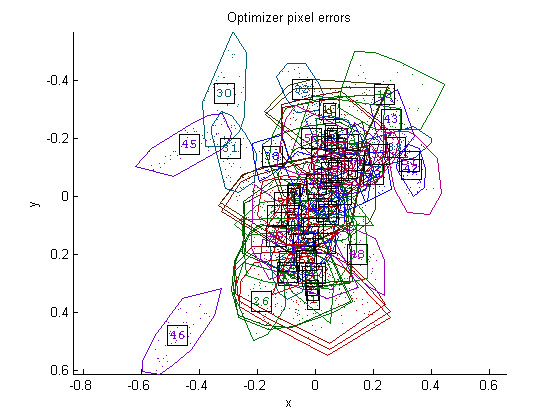
\includegraphics{figures/pixel_example}
\caption{Example output for \texttt{plotPixelErrors()}.}
\label{fig:pixel_example}
\end{figure}

This plots all reprojection errors, similar to Bouguet's \textsf{Analyse error} button.
Points are plotted as single pixels; the pixels for each observation get a single color,
a convex hull, and a label with the observation number at the centroid.
See Figure \ref{fig:pixel_example} for an example of output.

\begin{verbatim}
tree.plotExtrinsics();
\end{verbatim}

\begin{figure}[t]
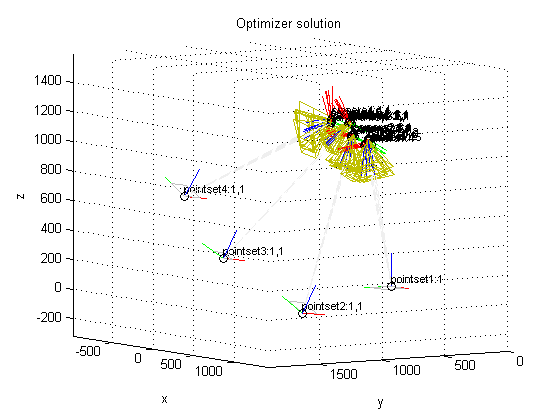
\includegraphics{figures/extrinsic_example}
\caption{Example output for \texttt{plotExtrinsics()}.}
\label{fig:extrinsic_example}
\end{figure}

This makes a 3-D plot (in the root frame) of camera and pointset transformations for each observation,
somewhat similar to Bouguet's \textsf{Show extrinsic} button, but accounting for 
the fact that there may be multiple cameras and/or pointsets.
See Figure \ref{fig:extrinsic_example} for an example of output.

\begin{verbatim}
tree.plotImagePoints();
\end{verbatim}

\begin{figure}[t]
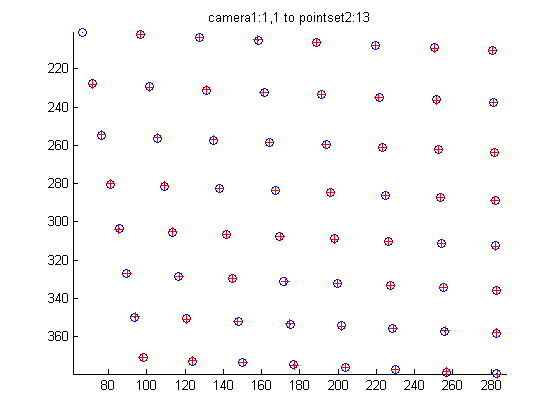
\includegraphics{figures/image_example}
\caption{Example output for \texttt{plotImagePoints()}.}
\label{fig:image_example}
\end{figure}

This makes one plot per observation of the observed image points and the reprojections of the solution.
See Figure \ref{fig:image_example} for an example of output. Note that the plots depend on the specific
observation types.

\begin{verbatim}
tree.relativeM('camera', Map({'main_arm', 'lamp_arm'}, {1, 2}), 'lamp_pointset');
\end{verbatim}

For the spherical gantry case, this gets the relative transformation between the camera and the lamp pointset 
when the main arm is in state 1 and the lamp arm is in state 2. You can specify a different set of node states for the pointset
with a fourth argument.



\part{API reference}
\section{I/O}

\subsection{\texttt{caliber.io.bouguet}: Bouguet calibration input}
\texttt{[ imagePoints, worldPoints, Q, data ] = bouguet( resultfile, indices )}
\paragraph{Overview.} This function reads a \texttt{Calib\_results.mat} file generated
by a Bouguet calibration and extracts the parameters for a single image.
Apart from this data, you will also need a tree structure to fully define the problem
to solve.
\paragraph{Inputs.}
\begin{itemize}
	\item \texttt{resultfile}: The name of a \texttt{Calib\_results.mat} generated
		by Bouguet.
	\item \texttt{indices}: The indices of the images within the file whose parameters are
		to be retrieved.
\end{itemize}
\paragraph{Outputs.}
\begin{itemize}
	\item \texttt{imagePoints}: A cell vector of $2 \times n$ arrays of observed image point coordinates.
	\item \texttt{worldPoints}: A cell vector of $3 \times n$ arrays of corresponding worldspace coordinates,
		in the pointset's frame.
	\item \texttt{Q}: A cell vector of estimated transformations between the camera and pointset frames.
    \item \texttt{data}: A struct containing intrinsic information for the camera.
\end{itemize}
\paragraph{Remarks.} 
	At current Bouguet is the only input format that we have specific code for.
	Note that Bouguet's convention has $z$ pointing in the direction that 
	the camera is looking, $y$ pointing downwards, and $x$ to the right from the
	camera's point of view.
\section{Tree}

\subsection{\texttt{caliber.initopt.tree}: problem defintion}
The \texttt{Tree} class is used to define the problem that you want Caliber to solve.
It is the class you will probably be working with the most.
\subsubsection{\texttt{Tree}: constructor}
\texttt{obj = Tree()}
\paragraph{Overview.}
The constructor creates a new \texttt{Tree} instance, which you then specify the problem to
using the \texttt{addNode} and \texttt{addObservation} methods, described next.
\paragraph{Inputs.}
None.
\paragraph{Outputs.}
\begin{itemize}
	\item \texttt{obj}: A new \texttt{Tree} instance.
\end{itemize}
\paragraph{Remarks.}

\subsubsection{\texttt{addNode}: add a node to the tree}
\texttt{addNode(node)}
\paragraph{Overview.}
This is one of two methods needed to specify a problem.
Generally you will add all the desired nodes before specifying observations.
\paragraph{Inputs.}
\begin{itemize}
	\item \texttt{Node}: The node object to add. Note that the first node that you add
		is the root of the tree.
\end{itemize}
\paragraph{Outputs.}
None.
\paragraph{Remarks.}
Nodes are not meant to be used in massive numbers--if you want to represent large pointsets, 
enter them as data on a single node and use an observation class such as \\ \texttt{caliber.observation.NodeObservation}.

\subsubsection{\texttt{addObservation}: add an observation to the tree}
\texttt{addObservation(observation, weight)}
\paragraph{Overview.} The other method needed to specify the problem.
\paragraph{Inputs.}
\begin{itemize}
	\item \texttt{observation}: The observation to add. See Section \ref{sec:observations} for details on constructing observations.
	\item \texttt{weight}: Optional. This controls the weight of the observation
		in the optimizer. If the weight is 0 it will not be used in finding the solution at all,
		which is useful for predictions and cross-validation. The default weight is 1.
\end{itemize}
\paragraph{Outputs.} None.
\paragraph{Remarks.}

\subsubsection{\texttt{solve}: solve the problem}
\texttt{[initializer, optimizer] = solve(tweaks, initializerOptions, optimizerOptions)}
\paragraph{Overview.}
After all nodes and observations have been added, this method attempts 
to find a solution.
\paragraph{Inputs.}
\begin{itemize}
	\item \texttt{tweaks}: Specifies what parameters are allowed to vary. 
		See Section \ref{sec:tweaks} for details.
	\item \texttt{initializerOptions}: Optional. 
		Options to feed to the initializer. Construct options using 
		\texttt{caliber.init.initializerOptionsSet}.
	\item \texttt{optimizerOptions}: Optional. 
		Options to feed to the internal \texttt{lsqnonlin} in the optimizer.
		Default options are \texttt{optimset('Jacobian', 'on', 'PlotFcns',
		 \{@plotOptResNormSemilogY; @plotOptStepSizeSemilogY\});}
\end{itemize}
\paragraph{Outputs.}
\paragraph{Inputs.}
\begin{itemize}
	\item \texttt{initializer}: An \texttt{Initializer} object that performed the initialization 
	stage of the problem solution. 
	See Section \ref{sec:initializer} for details.
	\item \texttt{optimizer}: An \texttt{Optimizer} object that performed the optimization 
	stage of the problem solution. 
	See Section \ref{sec:optimizer} for details.
\end{itemize}

\paragraph{Remarks.} Allowable options in \texttt{initializerOptionsSet} are:
\begin{itemize}
	\item \texttt{MaxDoFPerTransformation}: Maximum number of degrees of freedom for a single solved
		transformation. If the initializer cannot find a transformation which it can constrain
		the degrees of freedom below this number, it will report failure. Default is 6, 
		which will cause the initializer to guess $I$ for transformations if it cannot find 
		better information.
	\item \texttt{MaxDoFTotal}: The maximum total number of degrees of freedom in the initializer solution.
		If this amount would be exceeded, it will report failure. Default is \texttt{inf}, or no limit. 
	\item \texttt{SecondaryLabels}: The initializer can introduce new labels that represent products
		of transformations. This can lead to better solution strategies, though at computational cost.
		Allowed values are \texttt{'None'}, \texttt{'OneSide'} (the default), 
		\texttt{'BothSides'}, and \texttt{'All'}. The last in particular can be extremely expensive.
	\item \texttt{Tol}: A number representing how well-conditioned equations must be before the 
		initializer will consider a particular solution. Higher values result in more rejected
		equations. Default is 1e-3.
\end{itemize}

\subsubsection{\texttt{plotPixelErrors}: plot all reprojection errors}
\texttt{plotPixelErrors(predict)}
\paragraph{Overview.}
This plots all reprojection errors, much like Bouguet's \textsf{Analyse error}
button.
\paragraph{Inputs.}
\begin{itemize}
	\item \texttt{predict}: Optional. If true, it plots only for zero-weight 
		observations. Otherwise, it plots only for nonzero-weight observations.
\end{itemize}
\paragraph{Outputs.} None.
\paragraph{Remarks.}

\subsubsection{\texttt{plotExtrinsics}: 3-D plot of camera and pointset transformations}
\texttt{plotExtrinsics(predict)}
\paragraph{Overview.}
This makes a 3-D plot of camera and pointset transformations for each observation.
These are shown as frames where red, green, and blue lines represent the $x$, $y$,
and $z$ directions respectively.
\paragraph{Inputs.}
\begin{itemize}
	\item \texttt{predict}: Optional. If true, it plots only for zero-weight 
		observations. Otherwise, it plots only for nonzero-weight observations.
\end{itemize}
\paragraph{Outputs.} None.
\paragraph{Remarks.}

\subsubsection{\texttt{plotImagePoints}: plot image points and reprojections}
\texttt{plotImagePoints(predict)}
\paragraph{Overview.}
This makes a plot for each observation of the observed image points and their reprojections.
These are shown as blue circles and red crosses respectively; corresponding points
are connected by a black line.
\paragraph{Inputs.}
\begin{itemize}
	\item \texttt{predict}: Optional. If true, it plots only for zero-weight 
		observations. Otherwise, it plots only for nonzero-weight observations.
\end{itemize}
\paragraph{Outputs.} None.
\paragraph{Remarks.}

\subsubsection{\texttt{relativeM}: get the relative transformation between two nodes}
\texttt{M = relativeM(nodefrom, nodeto, statesfrom, statesto)}
\paragraph{Overview.}
This computes the relative transformation between two nodes given the current solution.
\paragraph{Inputs.}
\begin{itemize}
	\item \texttt{nodefrom}: The name of the node to compute the transformation from.
	\item \texttt{nodeto}: The name of the node to compute transformation to.
	\item \texttt{statesfrom}: A \texttt{containers.Map} mapping node names to state indices for \texttt{nodefrom}.
		Nodes with no explicitly specified state are assumed to be in their first state.
	\item \texttt{statesto}: Optional. A \texttt{containers.Map} mapping node names to state indices for \texttt{statesto}.
        Defaults to the same as \texttt{statesfrom}.
\end{itemize}
\paragraph{Outputs.}
\begin{itemize}
	\item \texttt{M}: The relative transformation from \texttt{nodefrom} to \texttt{nodeto},
		given node states defined by \texttt{statesfrom} and \texttt{statesto}.
\end{itemize}
\paragraph{Remarks.}

\subsubsection{\texttt{rootM}: get the transformation between the root and a node}
\texttt{M = rootM(node, states)}
\paragraph{Overview.}
This computes the relative transformation between the root and a node.
\paragraph{Inputs.}
\begin{itemize}
	\item \texttt{node}: The name of the node to compute the transformation to.
	\item \texttt{states}: A \texttt{containers.Map} mapping node names to state indices for \texttt{node}.
		Nodes with no explicitly specified state are assumed to be in their first state.
\end{itemize}
\paragraph{Outputs.}
\begin{itemize}
	\item \texttt{M}: The relative transformation from the root to \texttt{node},
		given node states defined by \texttt{states}.
\end{itemize}
\paragraph{Remarks.}

\subsubsection{\texttt{nodeM}: get the transformation of one state of a node}
\texttt{M = nodeM(node, stateIndex)}
\paragraph{Overview.}
This returns the transformation of one node in one state relative to its parent.
\paragraph{Inputs.}
\begin{itemize}
	\item \texttt{node}: The name of the node to compute the transformation on.
	\item \texttt{stateIndex}: Optional. The index of the state. Defaults to 1.
\end{itemize}
\paragraph{Outputs.}
\begin{itemize}
	\item \texttt{M}: The transformation of \texttt{node} in state with index \texttt{stateIndex}.
\end{itemize}
\paragraph{Remarks.}

\subsubsection{\texttt{nodeData}: get data associated with a node}
\texttt{data = nodeData(node, paramName)}
\paragraph{Overview.}
This returns data associated with a node.
\paragraph{Inputs.}
\begin{itemize}
	\item \texttt{node}: The name of the node which the data is associated with.
	\item \texttt{nodeData}: The name of the data to return, e.g. \texttt{'K'} for the camera matrix. 
\end{itemize}
\paragraph{Outputs.}
\begin{itemize}
	\item \texttt{data}: The data with that name at that node.
\end{itemize}
\paragraph{Remarks.}
\section{Tweaks}
\label{sec:tweaks}

\subsection{Tweak specification}

A tweak specification consists of a cell array, where each row contains four elements
that specify one or more parameters that are allowed to vary during the optimization.
Parameters are stored as matrices, which are themselves stored as elements of a \texttt{struct}.
These are \texttt{struct}s are the \texttt{data} member of \texttt{Node} classes.

\subsubsection{Node}
The first element in each row specifies which node contains the parameter to be tweaked.
This can be the name of the node, or a handle to the node itself.

\subsubsection{Parameter name}
The second element in each row specifies which field(s) of \texttt{node.data} can be modified.
This can be a string to specify a single field, or a cell array of strings to specify multiple 
fields at once.

\subsubsection{Parameter index(es)}
The third and fourth element in each row specifies which elements of \texttt{node.data.(parameterName)}
are allowed to vary. If the fourth element is empty, only the third element is used; otherwise the 
third element specifies the row and the fourth element the column. Both standard and logical indexing
are permitted; if you use logical indexing, remember to cast the indexing array to a logical array first.
You can also use the string \texttt{'all'}, which will select all elements (along that direction).

\subsection{Tweak objects}
Caliber uses the tweak specification to construct a \texttt{Tweak} object.

\paragraph{\texttt{tweak.node}}

A handle to the node that this tweak refers to.

\paragraph{\texttt{tweak.paramName}}

The parameter name that the tweak refers to. In other words, the tweak will
affect elements of \texttt{tweak.node.data.(tweak.paramName)}.

\paragraph{\texttt{tweak.paramIndices}}

This is a matrix whose nonzero elements indicate values of \\
\texttt{tweak.node.data.(tweak.paramName)} 
which are allowed to vary during the optimization. The value of the $j$th such element is equal to $j$.
For example, a camera matrix \texttt{'K'} whose focal length and principal point is allowed to vary
would have \texttt{tweak.paramIndices} equal to

\begin{center}\begin{tabular}{ccc}
    1 & 0 & 3 \\
    0 & 2 & 4 \\
    0 & 0 & 0
\end{tabular}\end{center}

For the extrinsic parameters \texttt{'r'} and \texttt{'t'}, the \texttt{tweak.paramIndices} are of the form

\begin{center}\begin{tabular}{c|cccc}
	& \multicolumn{4}{c}{Node states} \\
	& 1 & 2 & $\cdots$ & m \\
	\hline
	$x$ & ? & ? & $\cdots$ & ? \\
	$y$ & ? & ? & $\cdots$ & ? \\
	$z$ & ? & ? & $\cdots$ & ?
\end{tabular}\end{center}

\paragraph{\texttt{dValues = tweak.dValues()}}

Returns a cell array. The $j$th element of the array gives the derivative of 
\texttt{tweak.node.data} with respect to the $j$th nonzero element of \texttt{tweak.paramIndices}.
This turns out to be equal to \texttt{tweak.paramIndices ==} $j$.

\section{Nodes}
\label{sec:nodes}

\subsection{Provided node class}

\subsubsection{\texttt{GeneralNode}: standard 6-dimensional parameterization}

\texttt{node = GeneralNode( name, parentID, data, initialMs )}

\paragraph{Overview.} This node class represents a node with a list of transformations that
are each either completely known or completely unknown. It is appropriate for solving for 
general rigid transformations, such as robot arm links and rigid camera separations.

\paragraph{Inputs.}
\begin{itemize}
	\item \texttt{name}: The name of the node--this should be unique.
	\item \texttt{parentID}: Specifies the parent of the node. For the root node this should be empty.
	For other nodes, you can either refer to the parent by name or by handle.
	\item \texttt{data}: Data to associate with the node. This is a \texttt{struct} with matrices
	as fields.
	\item \texttt{initialMs}: A cell array of 4x4 transformation matrices representing the transformations
	associated with the states of this node. For an initially unknown transformation, use the empty matrix;
	this will be filled in by the initializer.
\end{itemize}
\paragraph{Remarks.}
\texttt{GeneralNode} parameterizes matrices relative to their initial value using 
\texttt{data.r} and \texttt{data.t}. Each of these is a $3 \times n$ matrix where each column represents
one state.

\subsection{Node methods}

If you wish to implement your own observation class, you will want to subclass \\
\texttt{caliber.node.Node}.
Then, you will need to implement several methods.

\subsubsection{Standard methods}

\paragraph{\texttt{dData = dData(tweak)}}

Does the same thing as \texttt{tweak.dValues()}.

\paragraph{\texttt{M = relativeM(stateIndices, targetNode, targetStateIndices)}}

Computes the relative transformation matrix between this node and another node.

\begin{itemize}
    \item \texttt{stateIndices}: The state indices of this node. 
        Generally you are calling this method on a camera node of an observation, so this argument should be \texttt{observation.cameraStateIndices}.
    \item \texttt{targetNode}: The target node. Usually this should be \texttt{observation.pointNode}.
    \item \texttt{targetStateIndices}: The state indices of the target node. Usually this should be \texttt{observation.pointStateIndices}.
\end{itemize}

\paragraph{\texttt{[dMs, tweakIndices] = dRelativeMs(stateIndices, targetNode, targetStateIndices, tweak)}}

This computes the derivative of M relative to the tweak parameters.

\begin{itemize}
    \item \texttt{stateIndices}: The state indices of this node. 
        Generally you are calling this method on a camera node of an observation, so this argument should be \texttt{observation.cameraStateIndices}.
    \item \texttt{targetNode}: The target node. Usually this should be \texttt{observation.pointNode}.
    \item \texttt{targetStateIndices}: The state indices of the target node. Usually this should be \texttt{observation.pointStateIndices}.
    \item \texttt{tweak}: The tweak in question.
\end{itemize}

\texttt{dMs} is a cell array and \texttt{tweakIndices} is a matrix, both with six elements. Each element \texttt{dMs\{j\}} gives the derivative of the 
transformation matrix between the two nodes with respect to the \texttt{tweakIndices(j)}th tweakable parameter of the tweak.
Elements of \texttt{dMs} may be empty matrices, indicating derivatives that are indentically zero; some \texttt{tweakIndices} may be
repeated, in which case the derivative is the sum of the corresponding elements of \texttt{dMs}.

\paragraph{\texttt{s = getStateString(stateIndices)}}

Gets a string representing the state of this node. May be useful for plot labels.
\begin{itemize}
    \item \texttt{stateIndices}: The state indices of this node. 
        Generally you are calling this method on a node of an observation, so this argument should be \texttt{observation.cameraStateIndices}
        or \texttt{observation.pointStateIndices}.
\end{itemize}

\subsubsection{Optional methods}
None currently.

\subsubsection{Required abstract methods}

\paragraph{\texttt{result = isKnown(obj, stateIndices)}}
Return true iff the transformation matrix is known for the specified state or all states.
If \texttt{stateIndices} has one element, return the answer for the \texttt{stateIndices}th element.
If \texttt{stateIndices} has more than one element, return the answer for the 
\texttt{stateIndices(obj.index)}th state.
(\texttt{obj.index} is automatically filled in when the object is assigned to a \texttt{Tree}).
If \texttt{stateIndices} is not given, return a logical array indicated which states have known 
transformation matrices.

\paragraph{\texttt{n = numberOfStates(obj)}}
Return the number of states associated with this node.

\paragraph{\texttt{M = getInitialM(obj, stateIndices)}}
Return the initial (i.e. pre-optimizer) transformation matrix of the \texttt{stateIndices(obj.index)}th state.

\paragraph{\texttt{setInitialM(obj, index, M)}}
Set the initial (i.e. pre-optimizer) transformation matrix of the \texttt{stateIndices(obj.index)}th state.
This is used by the initializer to set estimates for initially unknown transformations.

\paragraph{\texttt{M = M(obj, stateIndices)}}
Set the ``net'' transformation matrix (i.e. after parameters have been modified) of the \texttt{stateIndices(obj.index)}th state.

\paragraph{\texttt{[dMs, tweakIndices] = dMs(obj, state, tweak)}}
This should return the derivatives of the transformation matrix of this node for the given state
and the corresponding tweak indexes. You only need to return 
the derivatives that are nonzero as the cell array \texttt{dMs} and their corresponding tweak indexes 
as the array \texttt{tweakIndices}.

\section{Observations} \label{sec:observations}

\subsection{Provided observation classes}

A few observation classes are provided for conventional cameras.

\subsubsection{\texttt{IndependentObservation}: Observation of known 3-D points}

\texttt{observation = IndependentObservation( cameraName, pointName, imagePoints, worldPoints, Q, cameraStates, pointStates )}

\paragraph{Overview.} This observation class represents observations of 3-D points whose positions in the 
pointset frame are assumed to be perfectly known. It is appropriate for Bouguet-style observations.

\paragraph{Inputs.}
\begin{itemize}
	\item \texttt{cameraName}: The name of the camera node.
	\item \texttt{pointName}: The name of the pointset node.
    \item \texttt{imagePoints}: The observed image points, as a 2 x $n$ matrix.
    \item \texttt{worldPoints}: The corresponding world points (in the pointset node frame), as a 3 x $n$ matrix.
    \item \texttt{Q}: An estimate for the relative transformation from the camera node to the pointset node.
    \item \texttt{cameraStates}: A \texttt{containers.Map} mapping node names to state indices for the camera node. 
        Nodes with no explicitly specified state are assumed to be in their first state.
    \item \texttt{pointStates}: Optional. A \texttt{containers.Map} mapping node names to state indices for the pointset node. 
        Defaults to the same as \texttt{pointStates}.
\end{itemize}
\paragraph{Remarks.}

\subsubsection{\texttt{NodeObservation}: Observation of points assoicated with a node}

\texttt{observation = NodeObservation(cameraName, pointName, imagePoints, pointIndices, Q, cameraStates, pointStates) }

\paragraph{Overview.} This observation class represents observations of 3-D points whose positions 
may be shared between multiple observations and may not be perfectly known. 
This may be useful if you have point correspondences from a structure-from-motion algorithm.

\paragraph{Inputs.}
\begin{itemize}
	\item \texttt{cameraName}: The name of the camera node.
	\item \texttt{pointName}: The name of the pointset node. The pointset node should have a field \texttt{points} 
        in its \texttt{data} struct representing world points in that node's frame as a 3 x $n_\mathrm{max}$ matrix.
    \item \texttt{imagePoints}: The observed image points, as a 2 x $n$ matrix.
    \item \texttt{pointIndices}: A list of indices, which select $n$ columns of \texttt{pointNode.data.points} that 
        correspond to observed points.
    \item \texttt{Q}: An estimate for the relative transformation from the camera node to the pointset node.
    \item \texttt{cameraStates}: A \texttt{containers.Map} mapping node names to state indices for the camera node. 
        Nodes with no explicitly specified state are assumed to be in their first state.
    \item \texttt{pointStates}: Optional. A \texttt{containers.Map} mapping node names to state indices for the pointset node. 
        Defaults to the same as \texttt{pointStates}.
\end{itemize}
\paragraph{Remarks.}

\subsection{Implementing observation classes}

If you wish to implement your own observation class, you will want to subclass \\
\texttt{caliber.observation.Observation}.
Then, you will need to implement several methods.

\subsubsection{Optional methods}

\paragraph{\texttt{preSolve(obj, optimizer)}}

This is called before the optimizer calls \texttt{lsqnonlin}. 
This is a good place to do any precomputation or caching that affects the entire optimzation.
The default behavior is to query the optimizer for handles to the nodes with names
\texttt{obj.cameraNodeName} and \texttt{obj.pointNodeName},
and store them in \texttt{obj.cameraNode} and \texttt{obj.pointNode},
and to use \texttt{obj.cameraStates} and \texttt{obj.pointStates} to compute a vector 
that maps node indices to state indices in \texttt{obj.cameraStateIndices}
and \texttt{obj.pointStateIndices}. 
You will probably want to call \texttt{preSolve@super(obj, optimizer)}
if you override this method.

\paragraph{\texttt{plotImagePoints(obj)}}

If you implement this function, it should generate a plot of the image points for this observation.

\paragraph{\texttt{drawExtrinsics(obj, scale)}}

If you implement this function, it should draw a 3-D representation of the observation's extrinsics onto the current plot.
For example, you might draw three lines for the camera and pointset node frames representing their axes.
\texttt{scale} gives an idea of how large this representation should be.

\paragraph{\texttt{preIteration(obj)}}

This is called before each iteration of the optimizer, after all node data has been updated. This is a good place to 
do any precomputation or caching that affects a single iteration.

\subsubsection{Required abstract methods}

\paragraph{Constructor.}

Not technically an abstract method but worth mentioning. You will want to at least set the following inherited members:
\begin{itemize}
    \item \texttt{obj.cameraNodeName}: The name of the camera node.
    \item \texttt{obj.pointNodeName}: The name of the pointset node.
    \item \texttt{obj.cameraStates}: A \texttt{containers.Map} mapping node names to state indices for the camera node. 
        Nodes with no explicitly specified state are assumed to be in their first state.
    \item \texttt{obj.pointStates}: A \texttt{containers.Map} mapping node names to point indices for the camera node. 
        Nodes with no explicitly specified state are assumed to be in their first state.
\end{itemize}

\paragraph{\texttt{Q = getQ(obj)}}

This should return an estimate of the relative transformation between the camera and the pointset. Often you will
compute this externally, pass the estimate as an argument into the observation's constructor, then simply return it for this method.

\paragraph{\texttt{imagePoints = projectedImage(obj)}}

Compute the reprojection for the observation.

\paragraph{\texttt{imageError = reprojectionError(obj)}}

Compute the reprojection error for the observation. The output should be a column vector.

\paragraph{\texttt{errorJacobian = reprojectionErrorJacobian(obj, tweak)}}

Compute the Jacobian of the reprojection error for the observation with respect to the given tweak.
The output should be a matrix, preferably sparse. 
The $i$th row of the matrix corresponds to the $i$th element of the value that 
\texttt{reprojectionError} returns. The $j$th column of the matrix corresponds to the $j$th
nonzero value of \texttt{tweak.paramIndices}, and thus the matrix has a number of columns
equal to \texttt{nnz(tweak.paramIndices)}. 

For example, suppose \texttt{tweak.node} matches the camera node of the observation;  
\texttt{tweak.paramName} is \texttt{'K'}, or the camera matrix;
and \texttt{tweak.paramIndices} is

\begin{center}\begin{tabular}{ccc}
    1 & 0 & 3 \\
    0 & 2 & 4 \\
    0 & 0 & 0
\end{tabular}\end{center}

corresponding to the focal length and principal point parameters

\begin{center}\begin{tabular}{ccc}
    $f_x$ & - & $p_x$ \\
    - & $f_y$ & $p_y$ \\
    - & - & -
\end{tabular}\end{center}

Then the Jacobian for this tweak is

\begin{center}\begin{tabular}{c|cccc}
    & $f_x$ & $f_y$ & $p_x$ & $p_y$ \\
	\hline
	$x_1$ & $\frac{\partial x_1}{\partial f_x}$ & $\frac{\partial x_1}{\partial f_y}$ & $\frac{\partial x_1}{\partial p_x}$ & $\frac{\partial x_1}{\partial p_y}$ \\
	$y_1$ & $\frac{\partial y_1}{\partial f_x}$ & $\frac{\partial y_1}{\partial f_y}$ & $\frac{\partial y_1}{\partial p_x}$ & $\frac{\partial y_1}{\partial p_y}$ \\
	$x_2$ & $\frac{\partial x_2}{\partial f_x}$ & $\frac{\partial x_2}{\partial f_y}$ & $\frac{\partial x_2}{\partial p_x}$ & $\frac{\partial x_2}{\partial p_y}$ \\
	$y_2$ & $\frac{\partial y_2}{\partial f_x}$ & $\frac{\partial y_2}{\partial f_y}$ & $\frac{\partial y_2}{\partial p_x}$ & $\frac{\partial y_2}{\partial p_y}$ \\
	\vdots & \vdots & \vdots & \vdots & \vdots \\
	$x_n$ & $\frac{\partial x_n}{\partial f_x}$ & $\frac{\partial x_n}{\partial f_y}$ & $\frac{\partial x_n}{\partial p_x}$ & $\frac{\partial x_n}{\partial p_y}$ \\
	$y_n$ & $\frac{\partial y_n}{\partial f_x}$ & $\frac{\partial y_n}{\partial f_y}$ & $\frac{\partial y_n}{\partial p_x}$ & $\frac{\partial y_n}{\partial p_y}$
\end{tabular}\end{center}

where $\left( x_i, y_i \right)$ are the coordinates of the $i$th image point. Note that the order of the columns corresponds to the order of the nonzero
entries of \texttt{tweak.paramIndices}.

See Sections \ref{sec:tweaks} and \ref{sec:nodes} for details on accessing and computing 
tweak and node information.

\subsubsection{\texttt{StandardObservation}: conventional cameras}

If you are using a conventional camera, you may want to subclass \\
\texttt{caliber.observation.StandardObservation}
instead. This subclass implements most of the abstract methods of \\
\texttt{caliber.observation.Observation}, leaving
just the constructor and two new abstract functions to implement. 
Additionally, it caches the standard intrinsic and extrinsic parameters in \texttt{obj.M}, \texttt{obj.kc}, and \texttt{obj.K}
in \texttt{preIteration()} so you can look those up directly.

\paragraph{\texttt{points = getPoints(obj)}}

This method should return a set of 3-D points as a 3 x $n$ matrix.

\paragraph{\texttt{J = nonstandardJacobian(obj, tweak)}}

This method should compute the Jacobian of the image points with respect to a tweak
whose \texttt{paramName} is not one of \texttt{'K'}, \texttt{'kc'}, \texttt{'r'}, or \texttt{'t'}
(these cases are taken care of by \texttt{StandardObservation}).

\section{Initializer algorithm}

\subsection{Input and output}

Caliber consists of two stages. The first stage is the initializer, which considers the following 
input information:

\begin{itemize}
	\item A tree consisting of nodes $U$, with one node defined to be the root, and all other nodes
		having a single parent such that the root is the ultimate ancestor of all nodes.
	\item For each node $u$, an indexed set of states $u \colon 1 \ldots u \colon n$, 
		each with an associated
		rigid transformation $T_{u \colon i}$ relative to the node's parent. 
		This transformation may be initially known or unknown.
	\item A set of observations, defined by an estimated transformation $Q$ between a ``camera'' node
		and a ``pointset'' node, 
		a mapping $U \rightarrow \left\{u \colon 1 \ldots u \colon n \right\}$ defining 
		the state of the tree for the camera node, and another such mapping defining the state
		of the tree for the pointset node.
\end{itemize}

The result of the initializer is estimates for all initially unknown transformations $T_{u \colon i}$.

\subsection{State-expanded graph}

We do not solve the problem on the tree directly. Instead, we reduce the problem as stated
above to a problem that uses a \textit{state-expanded graph}. It is this problem that we will
call the initializer problem. An instance of this problem is defined as follows:
Given a set of vertices $V$ and a set of constraints, assign a rigid transformation $T_i$ to each vertex
such that all of the constraints are satisfied. (Define the first vertex to be the origin, so $T_0 = I$.)
Equivalently, if we imagine a complete graph, we wish to 
assign a rigid transformation to each ordered pair of vertices
(henceforth known as ``edges'') such that the constraints are satisfied, 
and the product of transformations around any cycle is the identity. 
It is this second formulation that we will use in our algorithm.

There are two types of expressible constraints in the initializer problem.

\paragraph{Direct constraint.} 
A constraint of this type restricts the transformation $T_{ij}$ 
on an edge to be a particular value.

\paragraph{Label constraint.} 
A constraint of this type restricts the transformations of a set of edges
to be equal to each other. Thus we can refer to this shared transformation as a label transformation.

\subsubsection{State expansion}

The state expansion that takes us from the tree representation to the state-expanded graph works as follows:

\begin{itemize}
	\item For each camera and pointset node and their respective states of each observation
		start at the root node and walk down the path to the camera or pointset node.
	\item For each node seen:
	\begin{itemize}
		\item Assign a graph vertex according to the following correspondence
		\begin{align}
			\text{tree node and a state index for each node on the path so far}
			\leftrightarrow \text{graph vertex}
		\end{align}
		\item Add a constraint between the previous graph vertex on the path and the current vertex.
			If the current node's state has a known transformation, create a direct constraint
			with that transformation.
			If the current node's state has a unknown transformation, create a label constraint
			with the following correspondence:
		\begin{align}
			\text{tree node and a state index for that node}
			\leftrightarrow \text{label}
		\end{align}
			Note that if we solve for the label transformation, we can easily write the result back
			into the original tree using this correspondence.
	\end{itemize}
	\item Finally, for each observation, add a direct constraint between 
	the camera and pointset graph vertices with the observation's estimated transformation.
\end{itemize}

Intuitively, the idea is that each vertex represents a point in the space of rigid transformations,
and the constraints reflect the knowledge about the relationships between these points that 
is implied by the tree. 

\subsubsection{Secondary labels}
In some cases, it may be easier to constrain the product of multiple labels and known transformations
than any single label. Therefore, we allow for the introduction of ``secondary labels''. 
Since there exists a unique path, and therefore a unique product of transformations, between any
two vertices in a tree, we can introduce a secondary label for every (symbolically) unique product
of transformations in the tree portion of the graph (i.e. all known and labeled edges in the graph,
excluding known edges that came from observations). Since known edges are handled by the direct rule,
we need only add secondary labels for paths that begin and end with edges with (primary) labels.

Finally, it is usually sufficient to consider only 
paths that are monotonically increasing in depth, which cuts down greatly on the number of secondary labels.

\subsection{Core algorithm}

With this problem reduction in hand, we can solve the problem on the graph to produce a solution 
for our original tree. To do this, we apply a series of rules, each of which may produce an estimate
of the transformation between some two vertices, until we have an estimate for every transformation
in the graph.

\subsubsection{Basic implications}

The condition that the product of transformations around any cycle must equal the identity has two
basic implications: $T_{ii} = I$ (each vertex frame is identical to itself), and $T_{ij} = T_{ji}^{-1}$
(the inverse transformation between two frames is defined by the inverse of the transformation matrix).
We do not consider these as distinct rules; instead we simply maintain these conditions when executing the
rules that follow.

\subsubsection{Direct rule}

The condition that the product of transformations around any cycle must equal the identity also gives rise
to our first rule, which we call the direct rule. It is sufficient to consider
only triangle-closing, by which we mean that if we have a length-2 path of known transformations, we
can estimate the transformation between the endpoints of the path as the product of those two transformations.
The transformation that closes a longer cycle can then be estimated by applying triangle-closing 
multiple times. Therefore, at the basic level, our direct rule performs this triangle-closing.

A pictorial representation of triangle closing:

\begin{align}
	\xymatrix{
	v_1 \ar[d]_A \ar@{-->}[dr]^{AB} & \\
	v_2 \ar[r]_B & v_3 
	}
\end{align}

Note that the arrows are only there to define which direction the transformation is referring to--this
has no bearing on the connectivity of the graph, since the opposite direction simply has the 
inverse of the transformation.

We can express the direct rule as a block matrix multiplication. We maintain a block matrix $T$ whose
blocks are 4x4 rigid transformations. The block $T_{ij}$ represents the rigid transformation
between vertices $i$ and $j$. Transformations that are currently unknown have $T_{ij} = 0$.
This is similar to an adjacency matrix, except instead of single binary entries indicating edges,
we have transformation matrix blocks.

The block elements of the product $T T = T^2$ are then:

\begin{align}
	T^2_{ij} = \sum_{k = 1}^n T_{ik} T_{kj} \approx n_{ij} T_{ij}
\end{align}

Each term in the sum is an estimate for the transformation $T_{ij}$ between $i$ and $j$ iff both 
$T_{ik}$ and $T_{kj}$ are nonzero (that is, known), and zero otherwise. 
$n_{ij}$ is the number of nonzero terms in the sum, 
which can be read out directly from the 
the bottom-right corner element (the homogeneous element) of $T^2_{ij}$. 
As long as at least one term in the sum is nonzero, 
$n_{ij} T_{ij}$ is in the same equivalence group as $T_{ij}$ since homogeneous coordinates are invariant 
to scaling.

\subsubsection{Label rule}

If the direct rule is unable to make progress, we move on to the label rule. We look through all the labels,
and if any of them has a edge with a known transformation, we set all other edges with the same label to
have the same transformation.

\subsubsection{AX = XB rule}

If neither of the previous rules can be applied, we use our final rule, which relies on solving 
systems of $AX = XB$ equations. After the direct rule is exhausted, every pair of vertices 
that has a path of known edges between them has a edge between them. 
Therefore, for every pair of edges with the same label $X$,
we can quickly check there exist known edges such that the cycle forms an $AX = XB$ equation.
Pictorially, the cycle corresponding to such an equation looks like this:

\begin{align}
	\xymatrix{
	v_1 \ar[d]_A \ar@{-->}[r]^{X} & v_3 \ar[d]_B \\
	v_2 \ar@{-->}[r]^{X}  & v_4 
	}
\end{align}

Since labels can potentially appear many times in the graph, there may be multiple such cycles,
each of which produces a different $AX = XB$ equation. Depending on the values of the $A$s and $B$s
and the number of equations, the solution space for each label may have a different number of dimensions.
In other words, some labels may be more constrained by their $AX = XB$ equations than others.
We choose the most constrained label in each step; if it does not yield a unique solution, we choose a
solution from the feasible space and report the number of degrees of freedom in the solution space.
We then return to the direct rule.

Note that this local analysis is not guaranteed to produce a correct solution even in case of exact 
measurements, 
nor to find a unique solution even if it exists. 
However, if it reports zero degree of freedom total, the solution is guaranteed to be unique correct.
In fact, we show later that the initializer problem is NP-hard, and it is also NP-hard to determine 
whether there exist multiple solutions. Therefore, unless P = NP, 
this implies that no polynomial-time algorithm
(which ours is) can guarantee a correct solution in all cases.

\subsection{Precision issues}
Since measurements will never be perfectly accurate and floating-point arithmetic has only finite precision,
in practice the problem and its solution. To address these issues, we use a least-squares solution at 
each step if there is additional information available, and in each $AX = XB$ case (described later),
we have some minimum tolerance for which we consider two vectors to be nonzero or nonparallel.


\section{Optimizer algorithm}

\subsection{Input and output}

The optimizer takes the output of the initializer, which is basically the initializer tree but with 
no unknown transformations, plus the following information:

\begin{itemize}
	\item For each node, a set of node data. This data can be any real matrices.
	\item For each observation, a reprojection error function and its Jacobian.
		For example, an conventional Bouguet-style observation's reprojection error
		function would take the relative transformation between the camera and pointset nodes
		and the intrinsics stored as the node data of the camera node, 
		compute the reprojected image points, and compare them to the actually observed points.
	\item A list of extrinsic parameters (rotation and translation of node states)
		and node data that is allowed to vary.
\end{itemize}

The optimizer then seeks a least-squares 
(in terms of the reprojection error across all observations) assignment of the parameters.

\subsection{Extrinsics}

\subsubsection{Parameterization}

An extrinsic parameter is defined by the following:

\begin{itemize}
    \item An edge state---changes to this parameter will change the transformation associated with that edge state.
    \item A parameter type, which for extrinsics is either rotation or translation.
    \item An axis---either $x$, $y$, or $z$.
\end{itemize}

We use the axis-angle representation for rotations. 
Rotations are special because the sum of two rotation vectors
does not in general produce a vector that represents the 
composition of the two rotations. Furthermore, the axis-angle 
representation is best-behaved near the identity. 
We parametrize the rotations as a second rotation relative
to the rotation produced by the initializer. Since we expect the 
initializer to produce a good estimate for the rotation, the 
second rotation should stay close to the identity throughout the 
optimization process.

\subsubsection{Evaluation}

Given a node state $s$, we can compute the transformation of that node relative
to the root $M_s$ by taking the product of the transformation of the edge states
defined by that node state on the path from the root to that node:

\begin{align}
    M_{\text{root} \rightarrow s} = 
    \prod_{\text{edges $i$ on path root $\rightarrow s$}} M_i
\end{align}

If we have
a camera node state $s$ and a pointset node state $t$, 
we can then find the relative pose
\begin{align}
    M_{s \rightarrow t} = M_s^{-1} M_t
\end{align}

\subsubsection{Jacobian}

A particular optimization parameter $x$ can only affect the extrinsics of an observation,
and by extension the extrinsics of its points, if both of the following hold:
\begin{itemize}
    \item The parameter is an extrinsic parameter. Intrinsic parameters do not affect extrinsics.
    \item The parameter refers to an edge state that is in the camera and/or pointset node state.
		Otherwise, the parameter
        refers to an entirely different camera and/or pointset node state, or to an edge that
		does not affect the pose of either the camera or pointset.
		Furthermore, if all edges above the closest common ancestor of the 
		two nodes have the same state
		in both the camera and pointset node states, and the parameter affects one of these edges,
		the parameter has the
		same effect on both the camera and pointset, and so does not affect the relative pose
		between the two.
\end{itemize}

If either of these does not hold, the derivative of the relative camera-pointset transformation
with respect to the parameter is zero.

If the parameter does affect the relative camera-pointset transformation, 
and all edges above the closest common ancestor of the two nodes have the same state
in both the camera and pointset node states, we need only consider edges 
on the path between the two nodes. 
In this case each edge is traversed only once, so we can simply replace the 
transformation of the affected edge state with its derivative:

\begin{align}
    \frac{dM_{s \rightarrow t}}{dx} = 
    \prod_{\text{edges $i$ on path $s \rightarrow t$}}
        \left\{ \begin{array}{ll}
            \frac{dT_i^{-1}}{dx} & \text{if edge is traversed towards root} \\
                & \text{and parameter refers to the edge state} \\
            \frac{dT_i}{dx} & \text{if edge is traversed away from root} \\
                & \text{and parameter refers to the edge state} \\
            T_i^{-1} & \text{if edge is traversed towards root} \\
                & \text{and parameter does not refer to the edge state} \\
            T_i & \text{if edge is traversed away from root} \\
                & \text{and parameter does not refer to the edge state}
        \end{array} \right.
\end{align}

The derivative of the inverse of a matrix can be expressed 
using the standard identity
\begin{align}
    \frac{dA^{-1}}{dx} = -A^{-1} \frac{dA}{dx} A^{-1}
\end{align}

In the more general case where the edges above the closest common ancestor of the two nodes
do not have the same states, we can find the derivatives of the product of transformations
from the root to the camera and pointset nodes $\frac{dM_s}{dx}$ and $\frac{dM_t}{dx}$,
then use the product rule to obtain
\begin{align}
    \frac{dM_{s \rightarrow t}}{dx} = \frac{dM_s^{-1}}{dx} M_t + M_s^{-1} \frac{dM_t}{dx}
\end{align}

\subsection{Node data (intrinsics)}

With the extrinsics settled, we now move on to node data, which can be used to describe
camera intrinsics, among other things.

\subsubsection{Parameterization}

We parameterize the elements of the node data matrices directly; any element of these 
matrices can be allowed to vary.

\subsubsection{Evaluation}

A particular observation reprojection function can take 
the relative transformation (or its Jacobian, for the Jacobian computation) as an input.
Typically, the reprojection function will then use node data from the camera node to 
compute the reprojection error.

\subsubsection{Jacobian}

Often the reprojection is a composition 
of functions of the form
\begin{align}
    \mathbf{y} & = f_i \left( \mathbf{x} \right)  \notag \\
    & = g_n \left( X_n, g_{n-1} \left( X_{n-1},  \ldots g_1 \left( X_1,  \mathbf{x} \right) \ldots \right) \right)
\end{align}
where the $j$th nested intrinsic function $g_j$ takes the result of the previous function $\mathbf{y}_{j-1}$ and 
uses it and some value $X_j$ to compute the result $\mathbf{y}_j$. 

In the conventional reprojection function we have the intrinsic functions outlined in Table \ref{tab:intrinsic_functions}.

\begin{table}[h]
    \begin{center}
        \caption{Intrinsic functions }
        \begin{tabular}{r|p{90mm}|p{25mm}}
            $j$ & $g_j$ & $X_j$ \\
            \hline
            1 & projection onto the image plane at unit distance in the camera's frame (multiplication by $M_s$ and division by the $z$ coordinate) & $M_s$ \\
            2 & radial distortion ($L$) & $\kappa = \left\{ \kappa_1, \kappa_2, \ldots \right\}$ \\
            3 & multiplication by the camera matrix ($K$) & $K$
        \end{tabular}
        \label{tab:intrinsic_functions}
    \end{center}
\end{table}

By the chain rule, and noting that each intrinsic parameter $x$ affects at most one of the values
$X_k$, the derivative of an intrinsic function with respect to $x$ is given by

\begin{align}
    \frac{d\mathbf{y}_{j}}{dx} & = \frac{d}{dx} g_j \left(X_j, \mathbf{y}_{j-1} \right) \\
    & = 
    \left\{ \begin{array}{ll}
        \frac{dg_j \left(X_j, \mathbf{y}_{j-1} \right)}{dX_j} \frac{dX_j}{dx} 
        & \text{if } k = j \\
        \frac{dg_j \left(X_j, \mathbf{y}_{j-1} \right)}{d\mathbf{y}_{j-1}} \frac{d\mathbf{y}_{j-1}}{dx} 
        & \text{if } k < j \\
        0 & \text{otherwise}
    \end{array} \right.
\end{align}

$\frac{dX_j}{dx}$ is typically a constant matrix, or in the case of the extrinsic matrix, 
computed as previously described.
$\frac{d\mathbf{y}_{j-1}}{dx}$ can be computed inductively, with the base case $\mathbf{y}_0$ 
referring to the observed points $\mathbf{x}$ themselves.

\section{Package structure}
For those of you interested in how the code is laid out, here is a summary of Caliber's package structure:

\subsection{Runnables}
These subpackages are the highest-level code and are generally run from the command line.
\subsubsection{\texttt{caliber.special}}
This package contains functions for calibrating particular types of configurations, such as rigid camera clusters.
\subsubsection{\texttt{test} subpackages}
Subpackages named ``\texttt{test}'' generally contain Caliber scripts or unit tests. Most are out of date.

\subsection{Core logic}
These subpackages implement the core logic of caliber.
\subsubsection{\texttt{caliber.tree}}
This subpackage contains the \texttt{Tree} class, which defines the problem description.
\subsubsection{\texttt{caliber.node}}
This subpackage contains the abstract \texttt{Node} class and its default implementation \texttt{GeneralNode}.
\subsubsection{\texttt{caliber.observation}}
This subpackage contains the abstract \texttt{Observation} class and some subclasses.
\subsubsection{\texttt{caliber.init}}
This subpackage contains the initializer code.
\subsubsection{\texttt{caliber.opt}}
This subpackage contains the optimizer code.

\subsection{Helper functions}
These packages contain mostly small functions that are used in other parts of caliber.
\subsubsection{\texttt{caliber.io}}
Functions here help process input to Caliber, or produce non-graphical output.
\subsubsection{\texttt{caliber.math}}
Various mathematical functions.
\subsubsection{\texttt{caliber.plot}}
Functions here deal with graphical output.


\part{Algorithm}
\section{I/O}

\subsection{\texttt{caliber.io.bouguet}: Bouguet calibration input}
\texttt{[ imagePoints, worldPoints, Q, data ] = bouguet( resultfile, indices )}
\paragraph{Overview.} This function reads a \texttt{Calib\_results.mat} file generated
by a Bouguet calibration and extracts the parameters for a single image.
Apart from this data, you will also need a tree structure to fully define the problem
to solve.
\paragraph{Inputs.}
\begin{itemize}
	\item \texttt{resultfile}: The name of a \texttt{Calib\_results.mat} generated
		by Bouguet.
	\item \texttt{indices}: The indices of the images within the file whose parameters are
		to be retrieved.
\end{itemize}
\paragraph{Outputs.}
\begin{itemize}
	\item \texttt{imagePoints}: A cell vector of $2 \times n$ arrays of observed image point coordinates.
	\item \texttt{worldPoints}: A cell vector of $3 \times n$ arrays of corresponding worldspace coordinates,
		in the pointset's frame.
	\item \texttt{Q}: A cell vector of estimated transformations between the camera and pointset frames.
    \item \texttt{data}: A struct containing intrinsic information for the camera.
\end{itemize}
\paragraph{Remarks.} 
	At current Bouguet is the only input format that we have specific code for.
	Note that Bouguet's convention has $z$ pointing in the direction that 
	the camera is looking, $y$ pointing downwards, and $x$ to the right from the
	camera's point of view.
\section{Initializer algorithm}

\subsection{Input and output}

Caliber consists of two stages. The first stage is the initializer, which considers the following 
input information:

\begin{itemize}
	\item A tree consisting of nodes $U$, with one node defined to be the root, and all other nodes
		having a single parent such that the root is the ultimate ancestor of all nodes.
	\item For each node $u$, an indexed set of states $u \colon 1 \ldots u \colon n$, 
		each with an associated
		rigid transformation $T_{u \colon i}$ relative to the node's parent. 
		This transformation may be initially known or unknown.
	\item A set of observations, defined by an estimated transformation $Q$ between a ``camera'' node
		and a ``pointset'' node, 
		a mapping $U \rightarrow \left\{u \colon 1 \ldots u \colon n \right\}$ defining 
		the state of the tree for the camera node, and another such mapping defining the state
		of the tree for the pointset node.
\end{itemize}

The result of the initializer is estimates for all initially unknown transformations $T_{u \colon i}$.

\subsection{State-expanded graph}

We do not solve the problem on the tree directly. Instead, we reduce the problem as stated
above to a problem that uses a \textit{state-expanded graph}. It is this problem that we will
call the initializer problem. An instance of this problem is defined as follows:
Given a set of vertices $V$ and a set of constraints, assign a rigid transformation $T_i$ to each vertex
such that all of the constraints are satisfied. (Define the first vertex to be the origin, so $T_0 = I$.)
Equivalently, if we imagine a complete graph, we wish to 
assign a rigid transformation to each ordered pair of vertices
(henceforth known as ``edges'') such that the constraints are satisfied, 
and the product of transformations around any cycle is the identity. 
It is this second formulation that we will use in our algorithm.

There are two types of expressible constraints in the initializer problem.

\paragraph{Direct constraint.} 
A constraint of this type restricts the transformation $T_{ij}$ 
on an edge to be a particular value.

\paragraph{Label constraint.} 
A constraint of this type restricts the transformations of a set of edges
to be equal to each other. Thus we can refer to this shared transformation as a label transformation.

\subsubsection{State expansion}

The state expansion that takes us from the tree representation to the state-expanded graph works as follows:

\begin{itemize}
	\item For each camera and pointset node and their respective states of each observation
		start at the root node and walk down the path to the camera or pointset node.
	\item For each node seen:
	\begin{itemize}
		\item Assign a graph vertex according to the following correspondence
		\begin{align}
			\text{tree node and a state index for each node on the path so far}
			\leftrightarrow \text{graph vertex}
		\end{align}
		\item Add a constraint between the previous graph vertex on the path and the current vertex.
			If the current node's state has a known transformation, create a direct constraint
			with that transformation.
			If the current node's state has a unknown transformation, create a label constraint
			with the following correspondence:
		\begin{align}
			\text{tree node and a state index for that node}
			\leftrightarrow \text{label}
		\end{align}
			Note that if we solve for the label transformation, we can easily write the result back
			into the original tree using this correspondence.
	\end{itemize}
	\item Finally, for each observation, add a direct constraint between 
	the camera and pointset graph vertices with the observation's estimated transformation.
\end{itemize}

Intuitively, the idea is that each vertex represents a point in the space of rigid transformations,
and the constraints reflect the knowledge about the relationships between these points that 
is implied by the tree. 

\subsubsection{Secondary labels}
In some cases, it may be easier to constrain the product of multiple labels and known transformations
than any single label. Therefore, we allow for the introduction of ``secondary labels''. 
Since there exists a unique path, and therefore a unique product of transformations, between any
two vertices in a tree, we can introduce a secondary label for every (symbolically) unique product
of transformations in the tree portion of the graph (i.e. all known and labeled edges in the graph,
excluding known edges that came from observations). Since known edges are handled by the direct rule,
we need only add secondary labels for paths that begin and end with edges with (primary) labels.

Finally, it is usually sufficient to consider only 
paths that are monotonically increasing in depth, which cuts down greatly on the number of secondary labels.

\subsection{Core algorithm}

With this problem reduction in hand, we can solve the problem on the graph to produce a solution 
for our original tree. To do this, we apply a series of rules, each of which may produce an estimate
of the transformation between some two vertices, until we have an estimate for every transformation
in the graph.

\subsubsection{Basic implications}

The condition that the product of transformations around any cycle must equal the identity has two
basic implications: $T_{ii} = I$ (each vertex frame is identical to itself), and $T_{ij} = T_{ji}^{-1}$
(the inverse transformation between two frames is defined by the inverse of the transformation matrix).
We do not consider these as distinct rules; instead we simply maintain these conditions when executing the
rules that follow.

\subsubsection{Direct rule}

The condition that the product of transformations around any cycle must equal the identity also gives rise
to our first rule, which we call the direct rule. It is sufficient to consider
only triangle-closing, by which we mean that if we have a length-2 path of known transformations, we
can estimate the transformation between the endpoints of the path as the product of those two transformations.
The transformation that closes a longer cycle can then be estimated by applying triangle-closing 
multiple times. Therefore, at the basic level, our direct rule performs this triangle-closing.

A pictorial representation of triangle closing:

\begin{align}
	\xymatrix{
	v_1 \ar[d]_A \ar@{-->}[dr]^{AB} & \\
	v_2 \ar[r]_B & v_3 
	}
\end{align}

Note that the arrows are only there to define which direction the transformation is referring to--this
has no bearing on the connectivity of the graph, since the opposite direction simply has the 
inverse of the transformation.

We can express the direct rule as a block matrix multiplication. We maintain a block matrix $T$ whose
blocks are 4x4 rigid transformations. The block $T_{ij}$ represents the rigid transformation
between vertices $i$ and $j$. Transformations that are currently unknown have $T_{ij} = 0$.
This is similar to an adjacency matrix, except instead of single binary entries indicating edges,
we have transformation matrix blocks.

The block elements of the product $T T = T^2$ are then:

\begin{align}
	T^2_{ij} = \sum_{k = 1}^n T_{ik} T_{kj} \approx n_{ij} T_{ij}
\end{align}

Each term in the sum is an estimate for the transformation $T_{ij}$ between $i$ and $j$ iff both 
$T_{ik}$ and $T_{kj}$ are nonzero (that is, known), and zero otherwise. 
$n_{ij}$ is the number of nonzero terms in the sum, 
which can be read out directly from the 
the bottom-right corner element (the homogeneous element) of $T^2_{ij}$. 
As long as at least one term in the sum is nonzero, 
$n_{ij} T_{ij}$ is in the same equivalence group as $T_{ij}$ since homogeneous coordinates are invariant 
to scaling.

\subsubsection{Label rule}

If the direct rule is unable to make progress, we move on to the label rule. We look through all the labels,
and if any of them has a edge with a known transformation, we set all other edges with the same label to
have the same transformation.

\subsubsection{AX = XB rule}

If neither of the previous rules can be applied, we use our final rule, which relies on solving 
systems of $AX = XB$ equations. After the direct rule is exhausted, every pair of vertices 
that has a path of known edges between them has a edge between them. 
Therefore, for every pair of edges with the same label $X$,
we can quickly check there exist known edges such that the cycle forms an $AX = XB$ equation.
Pictorially, the cycle corresponding to such an equation looks like this:

\begin{align}
	\xymatrix{
	v_1 \ar[d]_A \ar@{-->}[r]^{X} & v_3 \ar[d]_B \\
	v_2 \ar@{-->}[r]^{X}  & v_4 
	}
\end{align}

Since labels can potentially appear many times in the graph, there may be multiple such cycles,
each of which produces a different $AX = XB$ equation. Depending on the values of the $A$s and $B$s
and the number of equations, the solution space for each label may have a different number of dimensions.
In other words, some labels may be more constrained by their $AX = XB$ equations than others.
We choose the most constrained label in each step; if it does not yield a unique solution, we choose a
solution from the feasible space and report the number of degrees of freedom in the solution space.
We then return to the direct rule.

Note that this local analysis is not guaranteed to produce a correct solution even in case of exact 
measurements, 
nor to find a unique solution even if it exists. 
However, if it reports zero degree of freedom total, the solution is guaranteed to be unique correct.
In fact, we show later that the initializer problem is NP-hard, and it is also NP-hard to determine 
whether there exist multiple solutions. Therefore, unless P = NP, 
this implies that no polynomial-time algorithm
(which ours is) can guarantee a correct solution in all cases.

\subsection{Precision issues}
Since measurements will never be perfectly accurate and floating-point arithmetic has only finite precision,
in practice the problem and its solution. To address these issues, we use a least-squares solution at 
each step if there is additional information available, and in each $AX = XB$ case (described later),
we have some minimum tolerance for which we consider two vectors to be nonzero or nonparallel.


\section{AX = XB details}
\label{sec:ax-xb_details}

\subsection{Separation of rotation and translation}

It is sometimes useful to separate the $AX = XB$ equation on full rigid transformations into its translational
and rotational parts. This gives

\begin{align}
	R_A R_X = R_X R_B \label{eq:ax-xb_rotation} \\
	\left(R_A - I \right) t_x = R_X t_b - t_a \label{eq:ax-xb_translation}
\end{align}

\subsection{Screw axes}

It is also useful to observe that these equations describe a similarity transformation $B = X^{-1}AX$.
Furthermore, Chen \cite{Chen1991} gives a method of characterizing $AX = XB$ systems using 
screw theory. Briefly, screws are a way of representing rigid transformations. They consist of 
a screw axis, which is a line in space, a translation magnitude along that axis, and a 
rotation magnitude about that axis. Screws have the property that the translation and rotation magnitudes
are invariant with rigid transformations, whereas the screw axis transforms with rigid transformations.
Therefore, if we one or more $AX = XB$ equations, we can think of this problem as one where
we attempt to find the transformation $X$ that takes the screw axes given by $A_1, A_2, \ldots$ 
to those given by $B_1, B_2, \ldots$

\subsection{Cases with rotation}

\subsubsection{Nonparallel (skew or intersecting) screw axes (0 DoF)}

Park and Martin \cite{Park1994} give a method to compute the unique answer in the case where the 
screw axes are nonparallel and the rotation magnitudes are not near the identity or a 180-degree rotation 
(so the screw axes are well-defined). If the problem is overconstrained by having more than two $AX = XB$
equations, they give a least-square solution. In particular, they compute the rotational matrix that 
transforms a $3 \times n$ matrix of vectors $\alpha$ to another one $\beta$ as

\begin{align}
	M = \beta \alpha^T \\
	R = \left( M^T M \right)^{-\frac{1}{2}} M^T
\end{align}

\subsubsection{Parallel screw axes (1 DoF)}

Chen \cite{Chen1991} shows that in the case where the screw axes are parallel but not coincident, 
the rotation can be uniquely determined, but the translation has one degree of freedom.
For two such pairs of rigid transformations $A_1, B_1$ and $A_2, B_2$, 
we can construct an orthogonal using the (mutual)
screw axis direction, the direction separating the two screw axes, and their cross product.
We can then solve for the rotation as before. This is depicted in Figure \ref{fig:parallel-axis}.

\begin{figure}
\tdplotsetmaincoords{120}{60}
\begin{center}
\begin{tikzpicture}[tdplot_main_coords]
	\draw[->] (0,0,0) -- (0,0,4) node[anchor=north west]{$A_1$};
	\draw[->] (2,0,0) -- (2,0,4) node[anchor=north west]{$A_2$};
	\draw (0,0,1.5) -- (0.5,0,1.5);
	\draw (0.5,0,1) -- (0.5,0,1.5);
	\draw (0,0,1.5) -- (0,-0.5,1.5);
	\draw (0,-0.5,1) -- (0,-0.5,1.5);
	\draw (0.5,0,1) -- (0.5,-0.5,1);
	\draw (0,-0.5,1) -- (0.5,-0.5,1);
	\draw[dashed, ->] (0,0,1) -- (2,0,1);
	\draw[dashed, ->] (0,0,1) -- (0,-2,1);
	
	\tdplotsetrotatedcoords{40}{20}{70}
	\coordinate (Shift) at (5,5,0);
	\tdplotsetrotatedcoordsorigin{(Shift)}
	
	\draw[thick, shorten >=1cm,shorten <=2cm, ->] (0,0,1) -- (5,5,1) node[midway, above] {X};
	
	\draw[tdplot_rotated_coords, ->] (0,0,0) -- (0,0,4) node[anchor=north west]{$B_1$};
	\draw[tdplot_rotated_coords, ->] (2,0,0) -- (2,0,4) node[anchor=north west]{$B_2$};
	\draw[tdplot_rotated_coords] (0,0,1.5) -- (0.5,0,1.5);
	\draw[tdplot_rotated_coords] (0.5,0,1) -- (0.5,0,1.5);
	\draw[tdplot_rotated_coords] (0,0,1.5) -- (0,-0.5,1.5);
	\draw[tdplot_rotated_coords] (0,-0.5,1) -- (0,-0.5,1.5);
	\draw[tdplot_rotated_coords] (0.5,0,1) -- (0.5,-0.5,1);
	\draw[tdplot_rotated_coords] (0,-0.5,1) -- (0.5,-0.5,1);
	\draw[tdplot_rotated_coords, dashed, ->] (0,0,1) -- (2,0,1);
	\draw[tdplot_rotated_coords, dashed, ->] (0,0,1) -- (0,-2,1);
\end{tikzpicture}
\end{center}
\caption{Parallel screw axis frames.}
\label{fig:parallel-axis}
\end{figure}


Since $R_A$ always has at least one eigenvalue of unity, 
$\left(R_A - I \right)$ in the translation equation \ref{eq:ax-xb_translation} 
has a one-dimensional null space, and the solution space has one degree of freedom.
Since all the screws are parallel, this null space is the same for all of the equations.
In this case, we attempt to keep the translation as close to the origin as possible,
which we do by adding another row to the matrix $r_a' t_x = 0$.
Finally, we stack the equations produced by each pair of $AX = XB$ equations to produce a single
least-squares solution for $t_x$.

Note that this gives an alternate method for solving the skew screw axis case: choose one screw axis
as one direction, the direction along the shortest line between two screw axes as another, and their 
cross product as the third. Since in this case the null space of $\left(R_A - I \right)$ for
different equations are not the same, the translation has a unique solution.

\subsubsection{Coincident screw axes (2 DoF)}

In the coincident screw axis case, only one direction for the $A$s and for the $B$s can be determined;
in this case we choose the rotation axis to be along the (average) cross product of the screw axes,
which minimizes the rotation angle. We then solve for the translation as per the parallel axis case.

\subsection{Cases without rotation}

In some cases we may not have rotations at all; here the screw axis has direction equal to the translation
but its offset perpendicular to the axis direction is undefined. 
The rotation equation \label{eq:ax-xb_rotation} reduces to $R_X = R_X$, which gives us no information. 
The left side of the translation equation \ref{eq:ax-xb_translation} is zero, which means that $t_x$
cannot be determined at all, but there may be some information about $R_X$.

\subsubsection{Nonparallel translation (3 DoF)}

If the translations are nonparallel, we can use two non-parallel translations and their cross product to
determine the rotation uniquely, as in the noncoincident screw axis cases. 
As noted above, the translation is completely undetermined.

\subsubsection{Parallel translation case (4 DoF)}

Similarly, if we have only parallel translations, there is one degree of freedom. 
We can use the same method as the coincident screw axis case to determine a feasible rotation.
Again the translation is completely undetermined.

\subsubsection{No information case (6 DoF)}

If we have no information at all (no equations, or all $A$s and $B$s are the identity), then we
simply guess $X$ to be the identity.

\subsection{Omitted cases}

There are some cases which we have omitted here:

\subsubsection{180-degree rotations}

Chen \cite{Chen1991} addresses the case where some or all of the rotations are 180 degrees.
In these cases the rotation axis is defined, but only up to a binary choice between a direction
and its reverse.

\subsubsection{Mixed cases}

Chen \cite{Chen1991} also addresses the cases where different equations fall into different cases;
for example, one equation with rotation and one equation with only rotation. These cases
are amenable to the previous sort of analysis.

\subsubsection{Practical use}

We have not covered these cases so far because they are rare in practical use. Typically, the $A$s and $B$s
in the equations result from the relationship between two positions of a joint; this means 
skew screw axes for a ball joint (or equivalent, such as a spherical gantry), 
coincident screw axes for a revolute or cylindrical joint, and parallel translation for a prismatic joint;
and the changes in the estimated transformations from the corresponding observations.
Therefore, it is rare to find 180-degree rotations or mixed types of equations.
However, they could be added without too much difficulty.

\section{Initializer complexity}

\subsection{Binary choice via XAX = B}

The core gadget relies on cycles of the form $XAX = B$.

\subsubsection{Background}

\paragraph{Translation given rotations.}

Suppose we know the rotational part of $X$ but not the translational part--denote these by $R_X$ and $t_x$.
Then solving for the unknown $t_x$ reduces to
\begin{align}
	R_X R_A t_x + R_X t_a + t_x = t_b \\
	\left( R_X R_A + I \right) t_x = t_b - R_X t_a
\end{align} 
This has a unique solution as long as $R_X R_A + I$ is invertible. To see when this is the case,
consider this product for a unit vector $x$:
\begin{align}
	x^{-1} \left( R_X R_A + I \right) x = x^{-1} R_X R_A x + 1
\end{align}
For any rotation $R$, $x^{-1} R x$ is only $-1$ when $R$ is a 180-degree rotation.
Otherwise this shows that $R_X R_A + I$ is positive-definite and therefore invertible.
Thus it can be said that unless $R_X R_A$ is a 180-degree rotation, $t_x$ has a unique solution
given $R_X$.

\paragraph{Rotations.}
Inspiration taken from \\
\texttt{http://www.mathworks.com/matlabcentral/newsreader/view\_thread/165797}

From a single equation we have
\begin{align}
	XAX = B \\
	AXAX = AB \\
	AX = \left( AB \right)^\frac{1}{2}
\end{align}
Suppose we consider only the rotational part. 
The square root has multiple values; however, since our solution is restricted to 
$SO \left( 3 \right)$, this limits the possibilities.

\paragraph{The (more) undetermined case.}
If $R_A R_B = I$, then $I$ and any 180-degree rotation is a possible
square root. In our two-identical-tablet case, this would correspond to a situation 
where the two tablets have exactly anti-parallel camera axes.

\paragraph{The common case.}
Otherwise, $R_A R_B$ has a defined axis of rotation, 
and $\left( R_A R_B \right)^\frac{1}{2}$ must share that same axis, 
since applying any rotation twice preserves the axis of 
rotation. 
The magnitude of the rotation must be half that of $R_A R_B$,
plus an integer multiple of $\pi$. Since a difference of $2 \pi$ leaves the rotation matrix unchanged,
this produces two possible values for $\left( R_A R_B \right)^\frac{1}{2}$ and therefore two possible 
values for $R_X$.

\subsubsection{A special case}

\label{sec:special}
Let there exist some label $X$. Suppose we have a cycle that produces an $XAX = B$
equation. Let the rotational parts of $A$ and $B$ equal
\begin{align}
	R_A = R_B = \left[\begin{array}{ccc}
		0 &  -1 & 0 \\
		1 & 0 & 0 \\
		0 & 0 & 1
	\end{array} \right]
\end{align}

From this we have

\begin{align}
	R_X \in \left\{
		I,
		I'
	\right\} \\
	I = \left[\begin{array}{ccc}
			1 &  0 & 0 \\
			0 & 1 & 0 \\
			0 & 0 & 1
		\end{array} \right] \\
	I' = \left[\begin{array}{ccc}
			-1 &  0 & 0 \\
			0 & -1 & 0 \\
			0 & 0 & 1
		\end{array} \right]
\end{align}

Now let us examine the translational parts of $A$, $B$, and $X$. Suppose

\begin{align}
	t_a = \left[\begin{array}{c}
			0 \\ 0 \\ 0
		\end{array} \right] \\
	t_b = \left[\begin{array}{c}
			b \\ b \\ 0
		\end{array} \right]
\end{align}

for some constant $b$. In the case where $R_X = I$, we have

\begin{align}
	\left( R_X R_A + I \right) t_x = t_b - R_X t_a \\
	\left( R_A + I \right) t_x = t_b \\
	\left[\begin{array}{ccc}
		1 &  -1 & 0 \\
		1 & 1 & 0 \\
		0 & 0 & 1
	\end{array} \right] 
	t_x = \left[\begin{array}{c}
			b \\ b \\ 0
		\end{array} \right] \\
	t_x = \left[\begin{array}{c}
			b \\ 0 \\ 0
		\end{array} \right]
\end{align} 

In the case where $R_X = I'$, we have

\begin{align}
	\left( R_X R_A + I \right) t_x = t_b \\
	\left[\begin{array}{ccc}
		1 &  1 & 0 \\
		-1 & 1 & 0 \\
		0 & 0 & 1
	\end{array} \right] 
	t_x = \left[\begin{array}{c}
			b \\ b \\ 0
		\end{array} \right] \\
	t_x = \left[\begin{array}{c}
			0 \\ b \\ 0
		\end{array} \right]
\end{align}

Therefore, in this special case, $X$ either represents a step ``forwards'' of size $b$,
or a step to the left of size $b$ followed by an about-face. If $b = 0$, then the choice 
is between standing still and an about-face. Also note that if $b$ is an integer, all
arithmetic here is integer.

\subsection{Reduction from the (unique) partition problem}

We show a polynomial reduction from the (unique) partition problem to our initializer problem.

\subsubsection{The partition problem}

Recall the partition problem (PP). The definition of the problem is as follows:
given a set of positive integers $S = \left\{ x_1, x_2, \ldots x_n \right\}$, 
determine if there exists a subset of the integers $S_1$ such that
\begin{align}
	\sum_{x \in S_1} x = \sum_{x \not \in S_1} x
\end{align}

The standard form of the problem is well-known to be NP-complete; 
Dieudonne, et al. \cite{Dieudonne2010} show that, given an instance of this problem 
for which it is guaranteed that at least one solution exists, it is NP-hard
to determine whether there exists more than one solution.
They call this version the unique partition problem (UPP).

\subsubsection{The labeled transformation graph problem}

Now consider our initializer problem, which we will call the 
labeled transformation graph problem (LTGP).
The uniqueness version (ULTGP) of this problem asks whether, given an instance for LGTP which a solution
is guaranteed to exist, there exists more than one solution. (We consider swapping a particular choice
of $S_1$ with its complement in $S$ to be the same solution.)

\subsubsection{The core gadget}

Towards reducing PP to LTGP, we introduce the following gadget. For each $x_i \in S$, we introduce
two labels $X_i$ and $X_i'$. For both of these we construct an $XAX = B$ cycle of the form
described in Subsection \ref{sec:special}. For the one with $X_i$, we set $b = x_i$; for the one
with $X_i'$, we set $b = 0$. This produces four options for the product $X_i X_i'$, corresponding to 
our choice of picking $R_X = I$ or $R_X = I'$ for each rotational part:

\label{sec:steps}
\begin{enumerate}
	\item A step forward of size $x_i$ (choose $R_{X_i} = I$ and $R_{X_i'} = I$).
	\item A step forward of size $x_i$ followed by an about-face 
		(choose $R_{X_i} = I$ and $R_{X_i'} = I'$).
	\item A step left of size $x_i$ (choose $R_{X_i} = I'$ and $R_{X_i'} = I'$).
	\item A step left of size $x_i$ followed by an about-face (choose $R_{X_i} = I'$ and $R_{X_i'} = I$).
\end{enumerate}

We put one vertex of each such cycle at the root, so these are the only choices to be made here.
Since we do constant work per element of $S$, this stage is linear-time.

\subsubsection{A Manhattan walk}

With this set of gadgets in place, we introduce one more cycle, which we will treat as 
two paths from the root to a destination. On one side we constrain the transformation to the destination
to equal

\begin{align}
	T &= \left[\begin{array}{cccc}
			1 & 0 & 0 & \frac{1}{2} s \\
			0 & 1 & 0 & \frac{1}{2} s \\
			0 & 0 & 1 & 0 \\
			0 & 0 & 0 & 1
		\end{array} \right] \\
	\text{where} \ s &= \sum_i^n x_i
\end{align}

On the other side we have a path of $2n$ edges labeled such that they form the product 
\begin{align}
	T = \prod_i^n X_i X_i' = X_1 X_1' X_2 X_2' \ldots X_n X_n'
\end{align}

Again this is a linear-time transformation.

At each two-edge step towards the destination $X_i X_i'$ 
a solution must take one of the four options listed in Subsubsection \ref{sec:steps}.
This constrains our translations to lie only on cardinal directions. Since the Manhattan distance
to our target is $s$ and we only have a total of $s$ distance in translations in our product,
this means we must step towards the destination in every step. If we do an about-face 
before the last step, we will have to step away from the destination on the next step, and if 
we do an about-face on the last step, we will be facing the wrong direction. Therefore any solution must 
consist of only options 1 and 3. Since the forward steps total the same as the left steps in any solution,
this forms a one-to-one correspondence to a solution to PP--the indices of the steps in which we chose to move
forward correspond to the indices of the integers in the set we select to be in our partition.
Therefore PP reduces to LTGP, UPP reduces to ULTGP, and the initializer problem and its uniqueness version
are NP-hard.


\section{Optimizer algorithm}

\subsection{Input and output}

The optimizer takes the output of the initializer, which is basically the initializer tree but with 
no unknown transformations, plus the following information:

\begin{itemize}
	\item For each node, a set of node data. This data can be any real matrices.
	\item For each observation, a reprojection error function and its Jacobian.
		For example, an conventional Bouguet-style observation's reprojection error
		function would take the relative transformation between the camera and pointset nodes
		and the intrinsics stored as the node data of the camera node, 
		compute the reprojected image points, and compare them to the actually observed points.
	\item A list of extrinsic parameters (rotation and translation of node states)
		and node data that is allowed to vary.
\end{itemize}

The optimizer then seeks a least-squares 
(in terms of the reprojection error across all observations) assignment of the parameters.

\subsection{Extrinsics}

\subsubsection{Parameterization}

An extrinsic parameter is defined by the following:

\begin{itemize}
    \item An edge state---changes to this parameter will change the transformation associated with that edge state.
    \item A parameter type, which for extrinsics is either rotation or translation.
    \item An axis---either $x$, $y$, or $z$.
\end{itemize}

We use the axis-angle representation for rotations. 
Rotations are special because the sum of two rotation vectors
does not in general produce a vector that represents the 
composition of the two rotations. Furthermore, the axis-angle 
representation is best-behaved near the identity. 
We parametrize the rotations as a second rotation relative
to the rotation produced by the initializer. Since we expect the 
initializer to produce a good estimate for the rotation, the 
second rotation should stay close to the identity throughout the 
optimization process.

\subsubsection{Evaluation}

Given a node state $s$, we can compute the transformation of that node relative
to the root $M_s$ by taking the product of the transformation of the edge states
defined by that node state on the path from the root to that node:

\begin{align}
    M_{\text{root} \rightarrow s} = 
    \prod_{\text{edges $i$ on path root $\rightarrow s$}} M_i
\end{align}

If we have
a camera node state $s$ and a pointset node state $t$, 
we can then find the relative pose
\begin{align}
    M_{s \rightarrow t} = M_s^{-1} M_t
\end{align}

\subsubsection{Jacobian}

A particular optimization parameter $x$ can only affect the extrinsics of an observation,
and by extension the extrinsics of its points, if both of the following hold:
\begin{itemize}
    \item The parameter is an extrinsic parameter. Intrinsic parameters do not affect extrinsics.
    \item The parameter refers to an edge state that is in the camera and/or pointset node state.
		Otherwise, the parameter
        refers to an entirely different camera and/or pointset node state, or to an edge that
		does not affect the pose of either the camera or pointset.
		Furthermore, if all edges above the closest common ancestor of the 
		two nodes have the same state
		in both the camera and pointset node states, and the parameter affects one of these edges,
		the parameter has the
		same effect on both the camera and pointset, and so does not affect the relative pose
		between the two.
\end{itemize}

If either of these does not hold, the derivative of the relative camera-pointset transformation
with respect to the parameter is zero.

If the parameter does affect the relative camera-pointset transformation, 
and all edges above the closest common ancestor of the two nodes have the same state
in both the camera and pointset node states, we need only consider edges 
on the path between the two nodes. 
In this case each edge is traversed only once, so we can simply replace the 
transformation of the affected edge state with its derivative:

\begin{align}
    \frac{dM_{s \rightarrow t}}{dx} = 
    \prod_{\text{edges $i$ on path $s \rightarrow t$}}
        \left\{ \begin{array}{ll}
            \frac{dT_i^{-1}}{dx} & \text{if edge is traversed towards root} \\
                & \text{and parameter refers to the edge state} \\
            \frac{dT_i}{dx} & \text{if edge is traversed away from root} \\
                & \text{and parameter refers to the edge state} \\
            T_i^{-1} & \text{if edge is traversed towards root} \\
                & \text{and parameter does not refer to the edge state} \\
            T_i & \text{if edge is traversed away from root} \\
                & \text{and parameter does not refer to the edge state}
        \end{array} \right.
\end{align}

The derivative of the inverse of a matrix can be expressed 
using the standard identity
\begin{align}
    \frac{dA^{-1}}{dx} = -A^{-1} \frac{dA}{dx} A^{-1}
\end{align}

In the more general case where the edges above the closest common ancestor of the two nodes
do not have the same states, we can find the derivatives of the product of transformations
from the root to the camera and pointset nodes $\frac{dM_s}{dx}$ and $\frac{dM_t}{dx}$,
then use the product rule to obtain
\begin{align}
    \frac{dM_{s \rightarrow t}}{dx} = \frac{dM_s^{-1}}{dx} M_t + M_s^{-1} \frac{dM_t}{dx}
\end{align}

\subsection{Node data (intrinsics)}

With the extrinsics settled, we now move on to node data, which can be used to describe
camera intrinsics, among other things.

\subsubsection{Parameterization}

We parameterize the elements of the node data matrices directly; any element of these 
matrices can be allowed to vary.

\subsubsection{Evaluation}

A particular observation reprojection function can take 
the relative transformation (or its Jacobian, for the Jacobian computation) as an input.
Typically, the reprojection function will then use node data from the camera node to 
compute the reprojection error.

\subsubsection{Jacobian}

Often the reprojection is a composition 
of functions of the form
\begin{align}
    \mathbf{y} & = f_i \left( \mathbf{x} \right)  \notag \\
    & = g_n \left( X_n, g_{n-1} \left( X_{n-1},  \ldots g_1 \left( X_1,  \mathbf{x} \right) \ldots \right) \right)
\end{align}
where the $j$th nested intrinsic function $g_j$ takes the result of the previous function $\mathbf{y}_{j-1}$ and 
uses it and some value $X_j$ to compute the result $\mathbf{y}_j$. 

In the conventional reprojection function we have the intrinsic functions outlined in Table \ref{tab:intrinsic_functions}.

\begin{table}[h]
    \begin{center}
        \caption{Intrinsic functions }
        \begin{tabular}{r|p{90mm}|p{25mm}}
            $j$ & $g_j$ & $X_j$ \\
            \hline
            1 & projection onto the image plane at unit distance in the camera's frame (multiplication by $M_s$ and division by the $z$ coordinate) & $M_s$ \\
            2 & radial distortion ($L$) & $\kappa = \left\{ \kappa_1, \kappa_2, \ldots \right\}$ \\
            3 & multiplication by the camera matrix ($K$) & $K$
        \end{tabular}
        \label{tab:intrinsic_functions}
    \end{center}
\end{table}

By the chain rule, and noting that each intrinsic parameter $x$ affects at most one of the values
$X_k$, the derivative of an intrinsic function with respect to $x$ is given by

\begin{align}
    \frac{d\mathbf{y}_{j}}{dx} & = \frac{d}{dx} g_j \left(X_j, \mathbf{y}_{j-1} \right) \\
    & = 
    \left\{ \begin{array}{ll}
        \frac{dg_j \left(X_j, \mathbf{y}_{j-1} \right)}{dX_j} \frac{dX_j}{dx} 
        & \text{if } k = j \\
        \frac{dg_j \left(X_j, \mathbf{y}_{j-1} \right)}{d\mathbf{y}_{j-1}} \frac{d\mathbf{y}_{j-1}}{dx} 
        & \text{if } k < j \\
        0 & \text{otherwise}
    \end{array} \right.
\end{align}

$\frac{dX_j}{dx}$ is typically a constant matrix, or in the case of the extrinsic matrix, 
computed as previously described.
$\frac{d\mathbf{y}_{j-1}}{dx}$ can be computed inductively, with the base case $\mathbf{y}_0$ 
referring to the observed points $\mathbf{x}$ themselves.


%\bibliographystyle{plain}
%\bibliography{treecal-mail02}
\end{document}
